\documentclass[aspectratio=169,10pt]{beamer}
\usepackage[T1]{fontenc}
\usepackage{lmodern}
\usepackage{graphicx}
\usepackage{booktabs}
\usepackage{tabularx}
\usepackage{array}
\usepackage{xcolor}
\usepackage{hyperref}

\definecolor{lhcbgreen}{HTML}{16836B}
\definecolor{lhcbink}{HTML}{20303C}
\definecolor{lhcbmist}{HTML}{EEF3F5}
\setbeamercolor{structure}{fg=lhcbgreen}
\setbeamercolor{normal text}{fg=lhcbink,bg=white}
\setbeamercolor{frametitle}{fg=lhcbink,bg=white}
\setbeamercolor{block title}{fg=white,bg=lhcbgreen}
\setbeamercolor{block body}{fg=lhcbink,bg=lhcbmist}
\setbeamertemplate{navigation symbols}{}
\setbeamertemplate{footline}[frame number]
\setbeamersize{text margin left=8mm,text margin right=8mm}
\setlength{\tabcolsep}{5pt}
\renewcommand{\arraystretch}{1.17}

\title{LHCb Detector Acceptance Surfaces}
\subtitle{Reusable XY-plane geometries for transport and mask studies}
\author{Geometry builder documentation}
\date{17 October 2026}

\newcommand{\sourcepage}[2]{%
  \begin{frame}[plain]\centering
    \setbeamertemplate{footline}{}
    \makebox[\textwidth][c]{\includegraphics[page=#2,width=\paperwidth,height=\paperheight,keepaspectratio]{#1}}
  \end{frame}}

\begin{document}

\begin{frame}
  \titlepage
  \vspace{-2mm}
  \begin{center}\small Six lower-layout configurations; surfaces and fired-layer labels\end{center}
\end{frame}

\begin{frame}{Geometry payload and surface meaning}
\small
\begin{columns}[T,onlytextwidth]
  \column{0.52\textwidth}
  \begin{block}{What is stored}
    Each layout row names a detector surface, its logical layer/station label,
    its global $z$ in mm, and a Shapely XY geometry. Shapes are reusable pickle
    files; \texttt{detector\_setup.pickle} bundles the loaded layers and config.
  \end{block}
  \vspace{2mm}
  \textbf{Build chain}
  \begin{enumerate}
    \item Read placements and XY outlines from the ViewLHCb lower ROOT/GDML geometry.
    \item Convert outlines to polygons/unions and export named shape pickles.
    \item Record each plane's $z$ and logical label in \texttt{layout.csv}.
    \item Test each transported track crossing against the XY acceptance.
  \end{enumerate}
  \column{0.44\textwidth}
  \begin{block}{Important distinction}
    The masks are transverse acceptance surfaces, not a full material model.
    RICH is represented by projective entry/exit planes; PicoCal by two faces
    sharing an extracted footprint. The geometry does not model light transport,
    detailed material interactions, or the field map.
  \end{block}
  \vspace{2mm}
  \small Units are mm. The checked-in layout CSV is authoritative for plane
  names and exact $z$ values; summary tables round values for readability.
\end{columns}
\end{frame}

\begin{frame}{The six available lower configurations}
\small
\begin{tabularx}{\textwidth}{@{}c l c c X@{}}
\toprule
ID & UP border variant & SciFi T1/T2/T3 & UP XY envelope [mm] & SciFi XY envelope [mm] \\
\midrule
A & GDML nominal & 8/8/10 & 1394 $\times$ 1280 & 5652 $\times$ 4799 \\
B & Y8 top/bottom crop & 8/8/10 & 1394 $\times$ 965 & 5652 $\times$ 4799 \\
C & Y8X6 top/bottom + sides & 8/8/10 & 1165 $\times$ 965 & 5652 $\times$ 4799 \\
D & GDML nominal & 10/10/12 & 1394 $\times$ 1280 & 6707 $\times$ 4891 \\
E & Y8 top/bottom crop & 10/10/12 & 1394 $\times$ 965 & 6707 $\times$ 4891 \\
F & Y8X6 top/bottom + sides & 10/10/12 & 1165 $\times$ 965 & 6707 $\times$ 4891 \\
\bottomrule
\end{tabularx}

\vspace{4mm}
The six setup IDs are the Cartesian product of UP \texttt{gdml}, \texttt{y8},
\texttt{y8x6} and SciFi \texttt{8\_8\_10}, \texttt{10\_10\_12}.
TV, RICH1, MP, RICH2, PicoCal, and Muon are shared across the six choices.
The default catalog selection is UP Y8X6 with SciFi 8/8/10.
\end{frame}

\begin{frame}{UP variant XY surfaces and central hole}
\centering
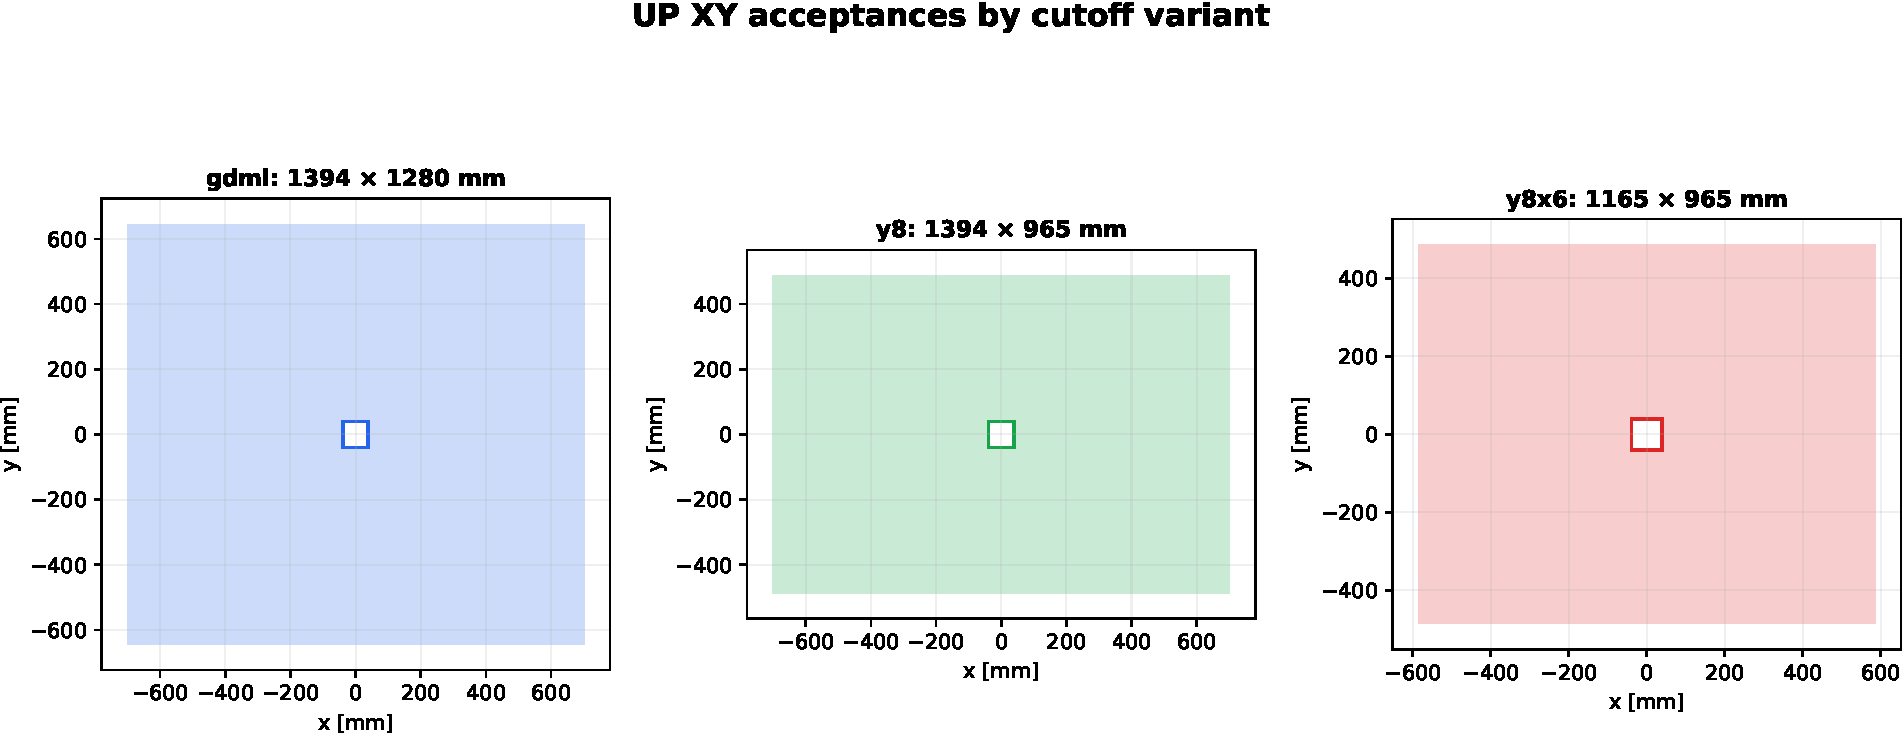
\includegraphics[page=1,width=0.96\textwidth,height=0.57\textheight,keepaspectratio]{assets/up_variant_comparison.pdf}
\vspace{1mm}
\small
\begin{tabularx}{0.96\textwidth}{@{}l X l@{}}
\toprule
Variant & Applied border crop & Central hole [mm] \\
\midrule
\texttt{UP\_GDML} & Nominal ViewLHCb/GDML borders & 77.3 $\times$ 79.9 \\
\texttt{UP\_Y8} & Remove 8 chips at top and bottom & 77.3 $\times$ 79.9 \\
\texttt{UP\_Y8X6} & Remove 8 top/bottom and 6 left/right chips & 77.3 $\times$ 79.9 \\
\bottomrule
\end{tabularx}
\end{frame}

\begin{frame}{How the acceptance outlines are derived}
\small
\begin{tabularx}{\textwidth}{@{}l l X@{}}
\toprule
Subsystem & Stored planes & Construction used in these setups \\
\midrule
TV / VELO & 50 & Pair nearby sensor-face groups within 2 mm in $z$; union each pair in XY. This yields one fired layer per TV layer. \\
RICH1/2 & 2 each & Project angular boundaries from the origin using $x=z\tan\theta_x$, $y=z\tan\theta_y$ at entry and exit $z$. Simplified planes only. \\
UP & 16 & Keep the extracted surfaces and group four consecutive surfaces per logical UP layer. Apply the selected border variant to XY. \\
MP & 5 & Union the extracted tile outlines into five logical XY layer surfaces, avoiding hundreds of per-tile planes. \\
SciFi / FT & 12 & Construct four X/U/V/X acceptance shapes at each T station; use module-count width, fixed height, central aperture, and stereo rotations. \\
PicoCal & 2 & Use the extracted front-region footprint as entry and exit faces spanning its $z$ extent. \\
Muon & 4 & Build a centered outer rectangle minus a centered rectangular beam aperture at M2--M5. \\
\bottomrule
\end{tabularx}

\vspace{3mm}
\footnotesize The generated surface views on the following slides are from the
selected setup's geometry summary. They show XY acceptance and Z placement;
they are not to scale across detector systems.
\end{frame}

\sourcepage{assets/reference_geometry_summary.pdf}{1}
\sourcepage{assets/reference_geometry_summary.pdf}{3}
\sourcepage{assets/reference_geometry_summary.pdf}{4}
\sourcepage{assets/reference_geometry_summary.pdf}{5}
\sourcepage{assets/reference_geometry_summary.pdf}{6}
\sourcepage{assets/reference_geometry_summary.pdf}{7}
\sourcepage{assets/reference_geometry_summary.pdf}{8}
\sourcepage{assets/reference_geometry_summary.pdf}{9}
\sourcepage{assets/reference_geometry_summary.pdf}{10}

\begin{frame}{SciFi module counts and stereo convention}
\begin{columns}[T,onlytextwidth]
  \column{0.53\textwidth}
  \begin{block}{Surface dimensions before rotation}
    Module width: 529.3 mm\\
    Active height: 4354 mm\\
    Central square opening: 260 $\times$ 260 mm\\[1mm]
    $W_x = 529.3 N$ mm, for $N \in \{8,10,12\}$
  \end{block}
  \smallskip
  T1 and T2 use the first module count in the selected triplet; T3 uses the
  third. For example, 8/8/10 means widths 4234.4, 4234.4, and 5293.0 mm.
  \column{0.43\textwidth}
  \begin{block}{Four surfaces per station}
    \begin{tabular}{@{}lrrr@{}}
    Layer & T1 $z$ & T2 $z$ & T3 $z$ [mm] \\
    X1 & 7902.700 & 8524.700 & 9209.700 \\
    U  & 7947.699 & 8569.699 & 9254.699 \\
    V  & 8032.701 & 8654.701 & 9339.701 \\
    X2 & 8077.700 & 8699.700 & 9384.700 \\
    \end{tabular}\\[1mm]
    Rotations: X1/X2 $0^\circ$, U $-5^\circ$, V $+5^\circ$.
  \end{block}
  \smallskip
  The exact $z$ coordinates are retained from extracted baseline X/U/V/X
  groups across all module-count choices. The layout CSV is authoritative.
\end{columns}
\end{frame}

\sourcepage{assets/six_configuration_comparison.pdf}{3}
\sourcepage{assets/six_configuration_comparison.pdf}{4}

\begin{frame}{Logical fired-layer labels}
\small
\begin{tabularx}{\textwidth}{@{}l c X@{}}
\toprule
Output & Range & Counting rule \\
\midrule
\texttt{nTV} & 0--50 & Number of paired-face TV layer unions crossed inside acceptance. \\
\texttt{nUP} & 0--4 & A logical layer fires if the crossing is inside the union of its four grouped source surfaces. \\
\texttt{nMP} & 0--5 & One hit per unioned MP layer. \\
\texttt{nFT} & 0--12 & One hit per X/U/V/X surface at T1, T2, and T3. \\
\texttt{nMuon} & 0--4 & One hit per M2, M3, M4, or M5 station. \\
\texttt{hasRich1Entry/Exit} & Boolean & Crossing inside the corresponding RICH1 face. Same convention for RICH2. \\
\texttt{hasRichEntry/Exit} & Boolean & OR of the corresponding entry/exit hit in RICH1 and RICH2. \\
\texttt{hasPicoCal} & Boolean & At least one of the two PicoCal faces is hit. \\
\bottomrule
\end{tabularx}

\vspace{4mm}
The loader can append a configuration label to output columns, for example
\texttt{nFT\_Run5}, so multiple setups can be evaluated on the same track.
Plane crossings are supplied by the transport/projector; this package tests
the crossing point against the selected XY shape and counts the fired labels.
\end{frame}

\begin{frame}{Provenance and files to use}
\small
\begin{itemize}
  \item \texttt{detector\_setups/catalog.json}: available choices and default setup.
  \item \texttt{detector\_setups/<setup>/config.json}: resolved setup options.
  \item \texttt{detector\_setups/<setup>/layout.csv}: exact plane names, labels, and global $z$ values.
  \item \texttt{detector\_setups/shared\_shapes/} and \texttt{up\_variants/}: reusable source shapes for the six catalog entries.
  \item \texttt{detector\_setups/<setup>/detector\_setup.pickle}: loaded geometry payload used by the mask loader.
\end{itemize}

\vspace{3mm}
\textbf{Scope note.} These are the current reusable acceptance configurations.
They are designed for geometry acceptance comparisons, not detector simulation.
The detailed plane definitions and saved XY shapes take precedence over the
rounded envelope dimensions shown in this deck.
\end{frame}

\end{document}
